\begin{problem}{Fiber Shape}{standard input}{standard output}{3 seconds}{512 megabytes}

Imagine a board with $n$ pins put into it, the $i$-th pin is located at $(x_i, y_i)$. 
For simplicity, we will restrict the problem to the case where the pins are placed in vertices of a convex polygon.

Then, take a non-stretchable string of length $l$, and put it around all the pins. Place a pencil inside the string and draw a curve around the pins, trying to pull the string in every possible direction. The picture below shows an example of a string tied around the pins and pulled by a pencil (a point $P$).

\begin{center}
\includegraphics{stmtfig.pdf}
\end{center}

Your task is to find an area inside this curve. Formally, for a given convex polygon $S$ and a length $l$ let's define a \emph{fiber shape} $F(S, l)$ as a set of points $t$ such that the perimeter of the convex hull of $S \cup \{t\}$ does not exceed $l$. Find an area of $F(S, l)$.

\InputFile
The first line contains two integers $n$ and $l$ ($3 \le n \le 10^4$; $1 \le l \le 8 \cdot 10^5$)~--- the number of vertices of the polygon $S$ and the length of the string. Next $n$ lines contain integers $x_i$ and $y_i$ ($-10^5 \le x_i, y_i \le 10^5$)~--- coordinates of polygon's vertices in counterclockwise order. All internal angles of the polygon are strictly less than $\pi$. The length $l$ exceeds the perimeter of the polygon by at least $10^{-3}$.

\OutputFile
Output a single floating-point number~--- the area of the fiber shape $F(S, l)$. Your answer will be considered correct if its absolute or relative error doesn't exceed $10^{-6}$. 

\Examples

\begin{example}
\exmpfile{example.01}{example.01.a}%
\exmpfile{example.02}{example.02.a}%
\exmpfile{example.03}{example.03.a}%
\end{example}

\Note
The following pictures illustrate the example tests.

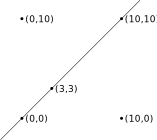
\includegraphics[scale=1.2]{sample1.pdf}
\includegraphics[scale=1.2]{sample2.pdf}


\begin{center}
\includegraphics[scale=1.6]{sample3.pdf}
\end{center}

\end{problem}

